\documentclass[a4paper,titlepage]{article}
\usepackage[utf8]{inputenc}
\usepackage{fullpage}
\usepackage{indentfirst}
\usepackage[per-mode=symbol]{siunitx}
\usepackage{listings}
\usepackage{graphicx}
\usepackage{color}
\usepackage{amsmath}
\usepackage{array}
\usepackage[hidelinks]{hyperref}
\usepackage[format=plain,font=it]{caption}
\usepackage{subcaption}
\usepackage{standalone}
\usepackage[nottoc]{tocbibind}
\usepackage[noabbrev,capitalize,nameinlink]{cleveref}
\usepackage{listings}
\usepackage{xspace}
\usepackage{tikz}
\usepackage{circuitikz}
\usepackage{titlesec}
\usepackage[cache=false]{minted}
\usepackage{booktabs}
\usepackage{csvsimple}
\newcommand{\MATLAB}{\textsc{Matlab}\xspace}
\usepackage{siunitx}
\usepackage[super]{nth}
\usepackage[titletoc]{appendix}

% Custom commands
\newcommand\numberthis{\addtocounter{equation}{1}\tag{\theequation}}
\newcommand{\code}[1]{\texttt{#1}}
\newcolumntype{P}[1]{>{\centering\arraybackslash}p{#1}}

\setminted{linenos,breaklines,fontsize=auto}

%\titleformat*{\section}{\normalsize\bfseries}
%\titleformat*{\subsection}{\small\bfseries}
\renewcommand{\thesubsection}{\thesection.\alph{subsection}}
\providecommand*{\listingautorefname}{Listing}
\newcommand*{\Appendixautorefname}{Appendix}

%opening
\title{\textbf{ECSE 543: Numerical Methods} \\ Assignment 1}
\author{Wenjie Wei \\ 260685967}
\date{\today}

\begin{document}
	\sloppy
	\maketitle
	
	\tableofcontents
	
	
	\twocolumn
	
	\section{Introduction}
	
	All programs in this assignment are written and compiled with Python 3.6. This report is structured so that the individual problems are answered in respective sections. The python codes used to solve the assignment problems are attached in the appendices, with the file names labeled at the top of the code segments.
	
	\section{Choleski Decomposition}
		\subsection{Choleski Implementation}
			The implementation of Choleski decomposition is shown in Listing \ref{lst:choleski}. There are two methods defined in \mintinline{python}{choleski.py}: \mintinline{python}{check_choleski(A, b, x)} and \mintinline{python}{choleski_decomposition(A, b)}. The latter method takes two matrices \mintinline{python}{A} and \mintinline{python}{b} as arguments, and returns \mintinline{python}{x} as the computational result of the decomposition. The first method takes these three matrices as arguments, and performs matrix production to check the result of
			$$
				Ax = b
			$$ 
			The precision of the equality is set to 0.001, as the program may end up with results with uncertainties with a quantity level of $10^{-8}$.
			
		\subsection{Simple Tester Matrices}
			To examine the functionality of the implementation, some tester matrices are constructed. The first tester matrix has randomly chosen entries, under the condition that the matrix is a non-singular, symmetric, positive definite matrix:
			$$
				\begin{bmatrix}
					15 & -5 & 0 & -5 \\
					-5 & 12 & -2 & 0 \\
					0 & -2 & 6 & -2 \\
					-5 & 0 & -2 & 9
				\end{bmatrix} x =
				\begin{bmatrix}
					115\\
					22\\
					-51\\
					13
				\end{bmatrix}
			$$
			
			To ensure non-singularity and positiveness, the entries on the primary diagonal must be chosen to be positive, otherwise the program with raise errors, meaning that the matrix does not meet the requirement. If the Choleski Decomposition succeeds, the matrix is proven to be positive definite.
			\begin{figure}[!h]
				\centering
				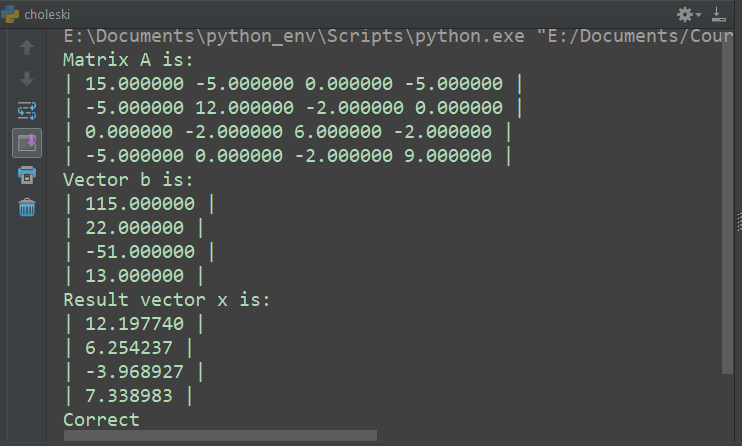
\includegraphics[width=\linewidth]{chol_1_result}
				\caption{Result of the First Choleski Decomposition Test}
				\label{chol_1_result}
			\end{figure}
		
			Figure \ref{chol_1_result} shows the result of the test of this certain tester matrix. This result is found to be correct by checking the dot product (which is implemented in file \mintinline{python}{matrix.py}) of matrix A and vector x. This result is also verified by \MATLAB using the back slash operator.
			
		\subsection{Linear Resistive Networks}
			Linear resistive networks are now able to be solved by the Choleski decomposition implemented in the previous parts. Listing \ref{lst:linear_networks} shows the implementation of reading a circuit file with data organized in a .csv file.
			
			\begin{figure}[!h]
				\centering
				\begin{circuitikz}[american voltages]
					\draw
					(0, 0) to [V, *-*] (0, 4)
					(0, 4) to [R, l=$20\Omega$, *-*] (3, 4) node[label={[font=\footnotesize]above:$V_1$}]{}
					to [R, l=$10\Omega$, *-*] (3, 2)node[label={[font=\footnotesize]left:$V_2$}]{}
					to [R, l=$30\Omega$, *-*] (6, 2)
					to [R, l=$30\Omega$, *-*] (6, 0)
					(3, 4) to [short, *-*] (6, 4)
					to [R, l=$10\Omega$, *-*] (6, 2)node[label={[font=\footnotesize]right:$V_3$}]{}
					(3, 2) to [R, l=$30\Omega$, *-*] (3, 0)
					to [short, *-*] (6, 0)
					to [short, *-*] (0, 0)
					(3, 0) node[ground]{}
					;
				\end{circuitikz}
				\caption{Test Circuit 5}
				\label{tc5}
			\end{figure}
			
			\begin{figure}[!h]
				\centering
				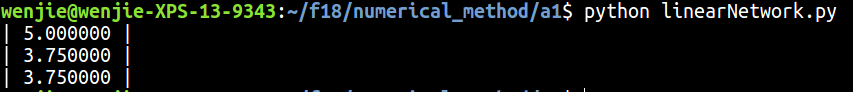
\includegraphics[width=\linewidth]{tc5_result}
				\caption{Result of the Testing Circuit 5}
				\label{tc5_result}
			\end{figure}
			
			Take the 5th circuit provided by the TA for example, the circuit is shown in Figure \ref{tc5}, and the result of the running of the program on this circuit is shown in Figure \ref{tc5_result}.
						
			The data of the circuit are organized in the way shown in Figure \ref{lin_network_org}.
			\begin{figure}[!h]
				\centering
				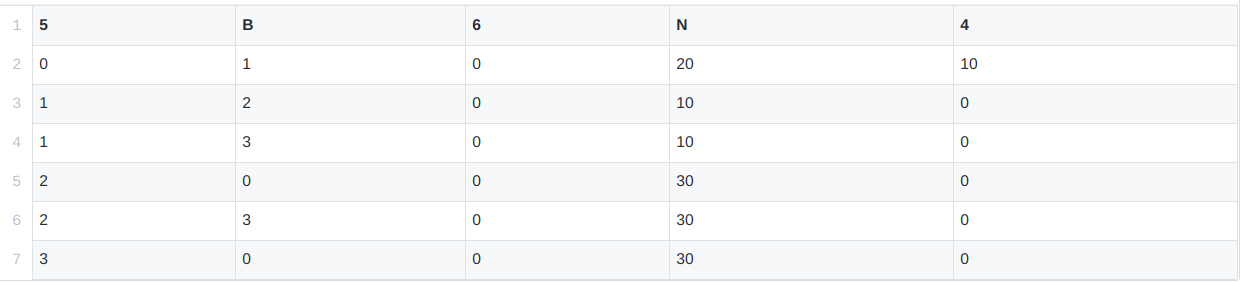
\includegraphics[width=\linewidth]{lin_network_org}
				\caption{Circuit File Organizations}
				\label{lin_network_org}
			\end{figure}
			The first line shows the general information about the circuit, such as the circuit ID (the example shown in the figure is the 5th test circuit), number of branches, and number of nodes. The lines followed are the data of the branches, which contains the following data: the starting node, the end node, the current source $J$, the resistance $R$, and the voltage source $E$.
			
			The convention of the input files should be well defined. In the program used for this test circuit, define the positive current direction is flowing from the start node to the end node. Current source must deliver positive current to the start node and the voltage source should deliver positive current to the end node. Following the conventions listed above, the program should be able to output desired node voltages in matrix form. 
			
			To verify the reliability of the program, four more simple test circuits are constructed. The input file as well as the result of the calculations are attached immediately after the circuit diagrams. The test runs below are proving that the program runs correctly as long as appropriate input files are passed into.
			\subsubsection{Testing Circuit 1}
				Figures \ref{tc1} and \ref{tc1_result} show the first test circuit. The desired output at node 1 can be calculated as $V_1 = 5V$, and the program is outputting the correct result.
				\begin{figure}[!h]
					\centering
					\begin{circuitikz}[american voltages]
						\draw
						(0, 0) to [V, l=$10V$, *-*] (0, 2)
						to [R, l=$10\Omega$, *-*] (2, 2) node[label={[font=\footnotesize]above:$V_1$}]{}
						to [R, l=$10\Omega$, *-*] (2, 0) node[ground]{}
						to [short, *-*] (0, 0)
						;
					\end{circuitikz}
					\caption{Test Circuit 1}
					\label{tc1}
				\end{figure}
				\begin{figure}[!h]
					\centering
					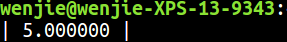
\includegraphics[width=\linewidth]{tc1_result}
					\caption{Output Result of the Testing Circuit 1}
					\label{tc1_result}
				\end{figure}
			\subsubsection{Testing Circuit 2}
				Figures \ref{tc2} and \ref{tc2_result} below show the testing circuit 2 and its result. The expected result is $V_1 = 50V$.
				\begin{figure}[!h]
					\centering
					\begin{circuitikz}[american voltages, american currents]
						\draw
						(0, 0) to [V, l=$10V$, *-*] (0, 2)
						to [short, *-*] (2, 2) node[label={[font=\footnotesize]above:$V_1$}]{}
						to [R, l=$10\Omega$, *-*] (2, 0) node[ground]{}
						to [short, *-*] (0, 0)
						(2, 0) to [short, *-*] (4, 0)
						to [I, i_>=$10A$, *-*] (4, 2)
						to [short, *-*] (2, 2)
						;
					\end{circuitikz}
					\caption{Test Circuit 2}
					\label{tc2}
				\end{figure}
				\begin{figure}[!h]
					\centering
					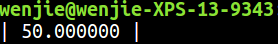
\includegraphics[width=\linewidth]{tc2_result}
					\caption{Output Result of the Testing Circuit 2}
					\label{tc2_result}
				\end{figure}
			\subsubsection{Testing Circuit 3}
				Figures \ref{tc3} and \ref{tc3_result} below show the results of the testing circuit 3. The expected result of the circuit is $V_1 = 55V$.
				\begin{figure}[!h]
					\centering
					\begin{circuitikz}[american voltages, american currents]
						\draw
						(0, 0) to [V, l=$10V$, *-*] (0, 2)
						to [R, l=$10\Omega$, *-*] (2, 2) node[label={[font = \footnotesize] above:$V_1$}]{}
						to [R, l=$10\Omega$, *-*] (2, 0) node[ground]{}
						to [short, *-*] (0, 0)
						(2, 0) to [short, *-*] (4, 0)
						to [I, i_>=$10A$, *-*] (4, 2)
						to [short, *-*] (2, 2)
						;
					\end{circuitikz}
					\caption{Test Circuit 3}
					\label{tc3}
				\end{figure}
				\begin{figure}[!h]
					\centering
					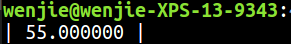
\includegraphics[width=\linewidth]{tc3_result}
					\caption{Output Result of the Testing Circuit 3}
					\label{tc3_result}
				\end{figure}
			\subsubsection{Testing Circuit 4}
				Figures \ref{tc4} and \ref{tc4_result} below show the results of the testing circuit 4. The expected results of the circuit is $V_1 = 20V$ and $V_2 = 35V$.
				\begin{figure}[!h]
					\centering
					\begin{circuitikz}[american voltages, american currents]
						\draw
						(0, 0) to [V, l=$10V$, *-*] (0, 2)
						to [R, l=$10\Omega$, *-*] (2, 2) node[label={[font = \footnotesize] above:$V_1$}]{}
						to [R, l=$5\Omega$, *-*] (4, 2) node[label={[font = \footnotesize] above:$V_2$}]{}
						to [R, l=$5\Omega$, *-*] (4, 0) node[ground]{}
						to [short, *-*] (2, 0)
						to [R, l=$10\Omega$, *-*] (2, 2)
						(2, 0) to [short, *-*] (0, 0)
						(4, 0) to [short, *-*] (6, 0)
						to [I, i_>=$10A$, *-*] (6, 2)
						to [short, *-*] (4, 2)
						;
					\end{circuitikz}
					\caption{Test Circuit 4}
					\label{tc4}
				\end{figure}
				\begin{figure}[!h]
					\centering
					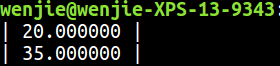
\includegraphics[width=\linewidth]{tc4_result}
					\caption{Output Result of the Testing Circuit 4}
					\label{tc4_result}
				\end{figure}
								
	\onecolumn
	\begin{appendices}
		
		\section{Code Listings} \label{appendix:code}
		
		\setminted{linenos,breaklines,fontsize=\footnotesize}
		
		\begin{center}
			\captionof{listing}{Custom matrix package (\texttt{matrix.py}).}
			\inputminted{python}{../matrix.py}
			\label{lst:matrices}
		\end{center}
		
		\begin{center}
			\captionof{listing}{Choleski decomposition (\texttt{choleski.py}).}
			\inputminted{python}{../choleski.py}
			\label{lst:choleski}
		\end{center}
		
		\begin{center}
			\captionof{listing}{Linear resistive networks (\texttt{linear\_networks.py}).}
			\inputminted{python}{../linearNetwork.py}
			\label{lst:linear_networks}
		\end{center}
		
	\end{appendices}
	

\end{document}